\documentclass{article}
\usepackage{graphicx}
\usepackage{amsmath}
\usepackage{float}
\usepackage{mathtools}
\usepackage{subcaption}
\graphicspath{ {./photos/} }
\title{Passion Project}
\author{Nicola Ouzounov}
\date{January 2026}

\begin{document}

\maketitle
\tableofcontents

\section{Introduction}
This is a passion project of mine, where I go out of my way to educate myself.
I have been reading about numerical differentiation, approximation etc.
Based on the things, that I have read, I am making programs with no real application, other than to get acquainted with numerical methods.
My goal is that this knowledge will come in help later down the line in my educational/professional life.
With that in mind this document will contain information about the different programs, that I have made, and maybe some comments about the work, put in them.\\
\section{Euler Approximation Method}
This method is used to numerically solve first order differential equations of this type: $y' = f(x, y)$.
Using the following property of the derivative we can approximate the original function for very small intervals $x - x_0 = h \rightarrow0$:
\begin{equation*}
    y'(x) = lim_{x\rightarrow x_0}\frac{y(x) - y(x_0)}{x-x_0}
\end{equation*}
\begin{equation*}
    \Rightarrow y(x) \approx y'(x)*(x-x_0) + y(x_0)
\end{equation*}
\begin{equation*}
    \Rightarrow y(x) \approx f(x, y) *(x-x_0) + y(x_0)
\end{equation*}
Therefore if we use the given to us function $f(x, y)$ and the initial condition for example $y(0) = y_0$, we can evaluate the next value $y_1, y_2, ...$ etc. Let us take a look at the following example:
\begin{equation*}
    y' - y = -\frac{1}{2}e^{x/2}sin(5x) + 5e^{x/2}cos(5x)
\end{equation*}
\begin{equation*}
    \Rightarrow f(x, y) = y -\frac{1}{2}e^{x/2}sin(5x) + 5e^{x/2}cos(5x)
\end{equation*}
\begin{equation*}
    \Rightarrow y_{n+1} = y_n + f(t_n, y_n)(t_{n+1} - t_n);
\end{equation*}
When put into a MATLAB script, we will make the following boundaries, in order to form a visualization:
\begin{itemize}
    \item The initial given value is $y(1) = 0$.
    \item The graph takes place in $x \in [0, 10]$.
    \item The step size is $h = 0.05$.
\end{itemize}
\begin{figure}[H]
    \centering
    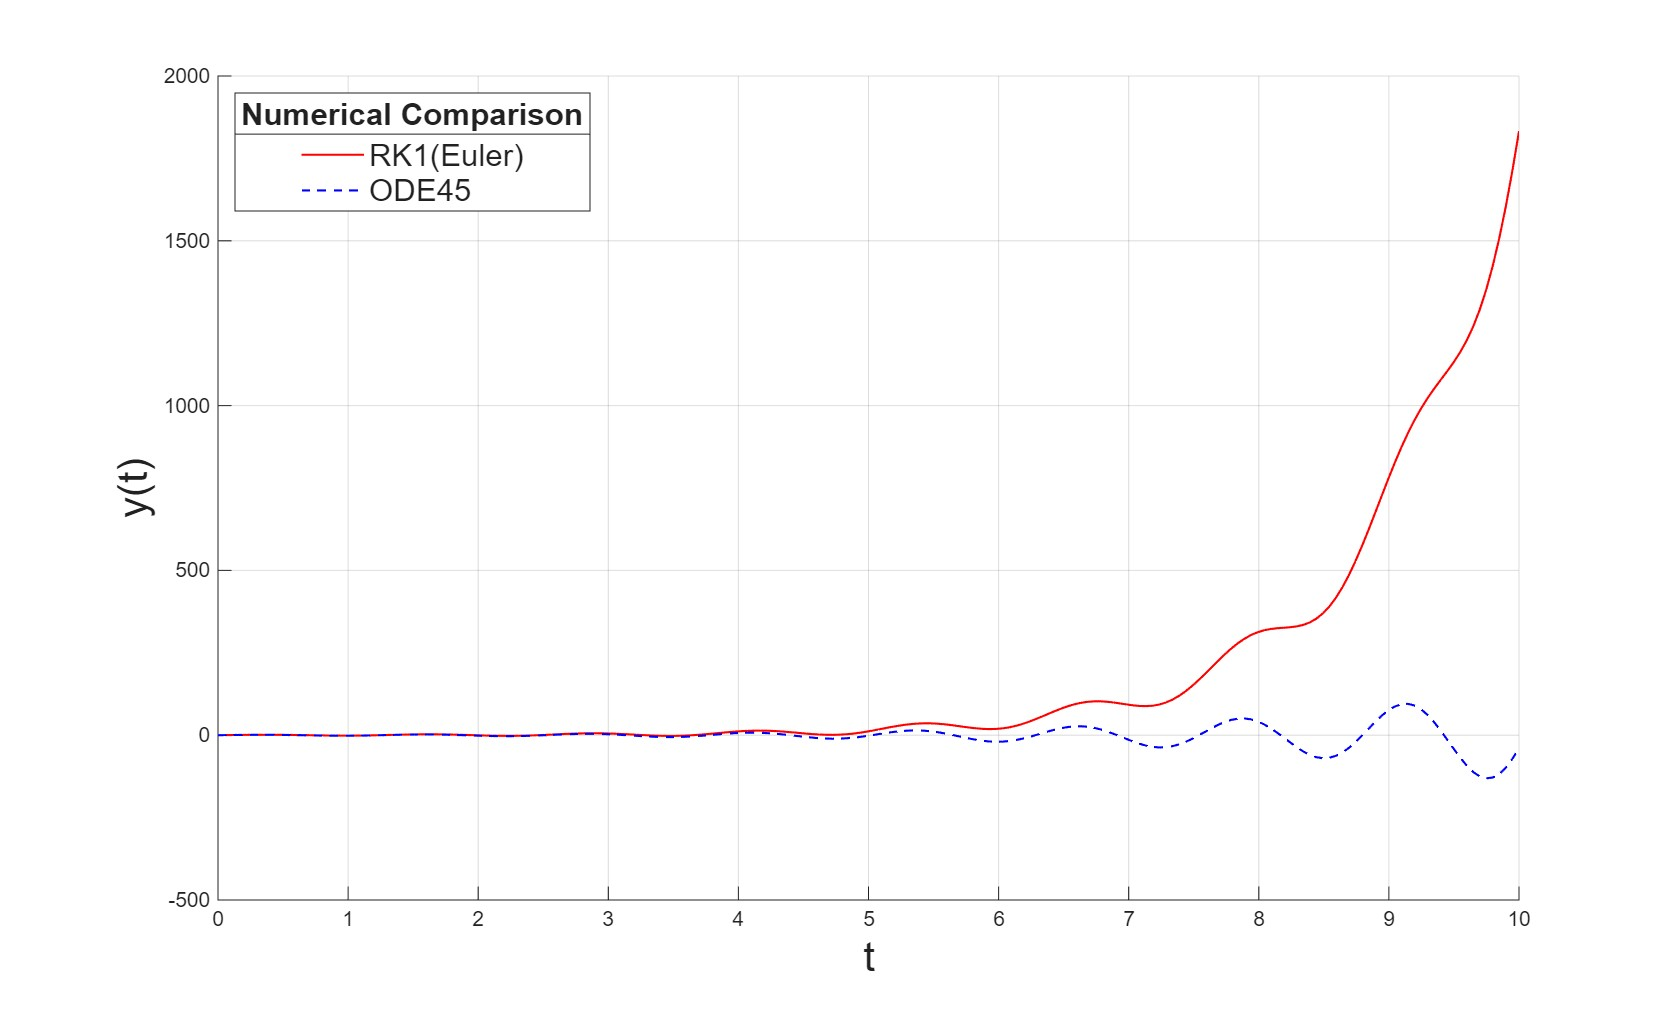
\includegraphics[width=1\linewidth]{rk1_005.jpg}
    \caption{RK1, h = 0.05}
    \label{fig:rk1_005}
\end{figure}
As we can see from this image, the method is not converging fast enough. If we make the step size even smaller it converges, of course. To calculate the error, we can simply find the difference between Euler and ODE45. Then the difference is plotted with respect to t:
\begin{figure}[H]
    \centering
    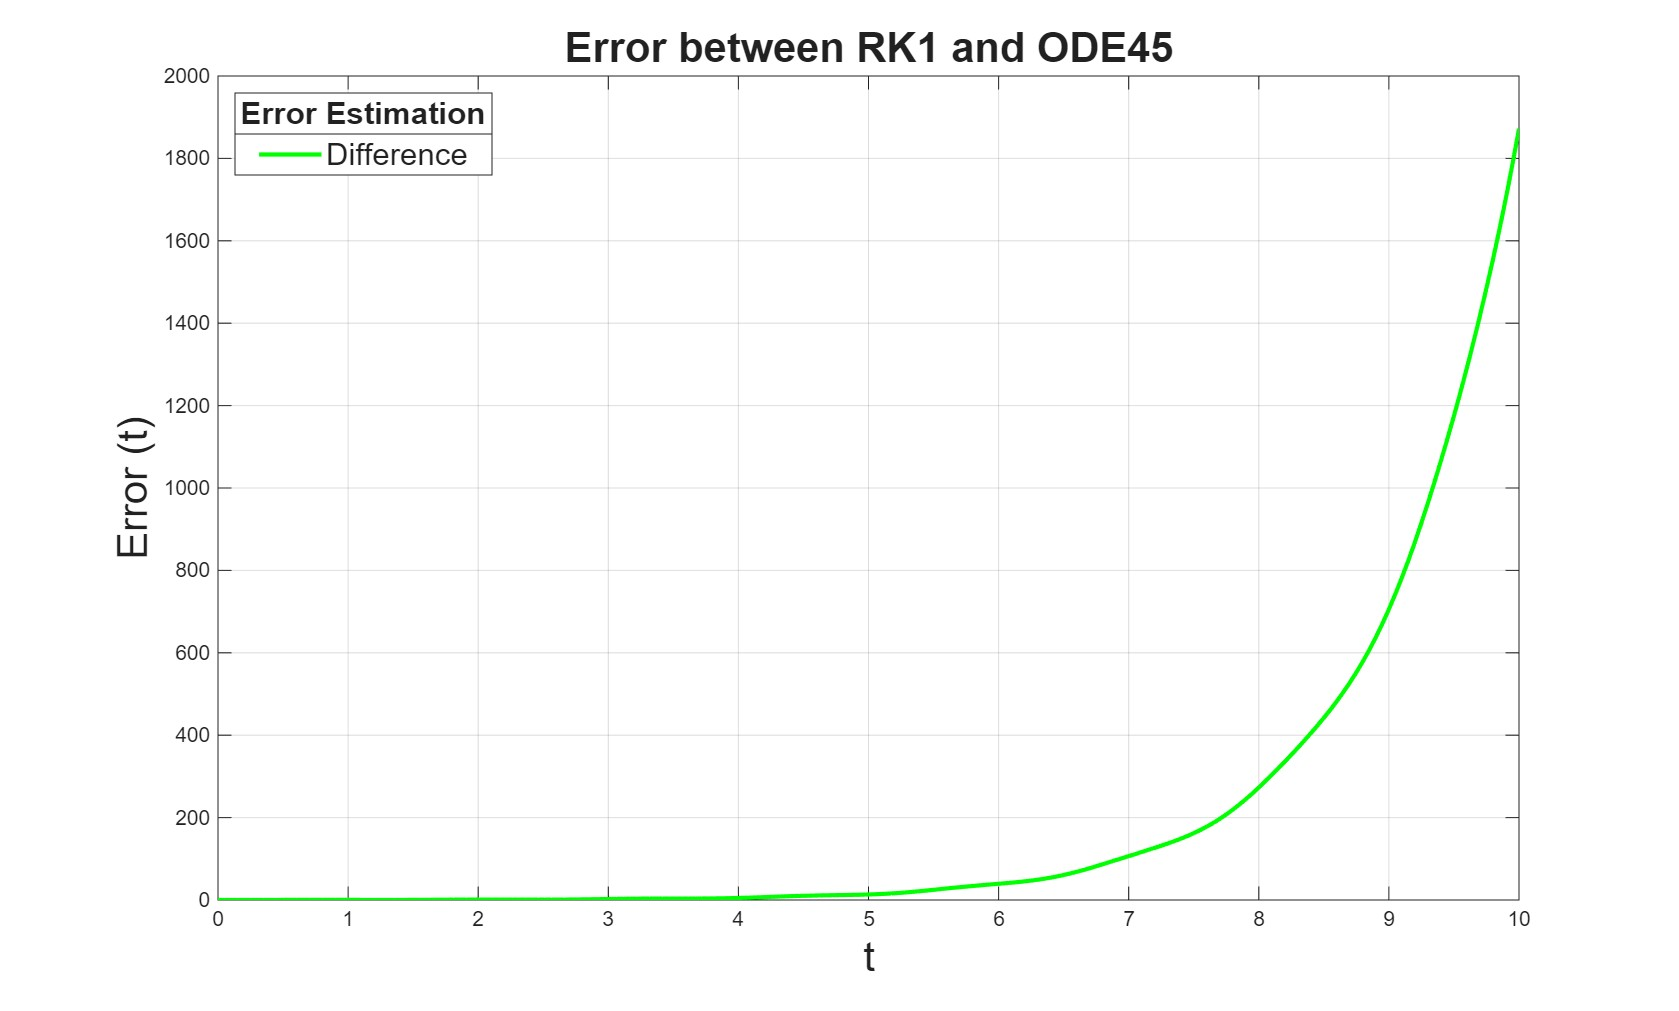
\includegraphics[width=1\linewidth]{error_rk1.jpg}
    \caption{Error Euler}
    \label{fig:error_rk1}
\end{figure}
From the original graph of both solutions and from this one it is obvious that the solution is not good at all.
\section{RK2 Method}
In this section I am introducing the RK2 and RK4 method. We are approximating the same function as in the Euler section, but this time it is compared not to the analytical solution but to the MATLAB function ODE45. The assumptions in place:
\begin{itemize}
    \item $f(x,y) =  y -\frac{1}{2}e^{x/2}sin(5x) + 5e^{x/2}cos(5x)$
    \item Initial Value Condition $y(0) = 0$
    \item The step size is $h = 0.05$
\end{itemize}
Similar to the Euler's Method we will calculate numerically the solution. The difference this time is the accuracy. By Euler's Method the error is $\sim h$. By RK2 the error is $\sim h^2$. The way the RK2 is implemented looks as follows:
\begin{align*}
    A = f(x_n, y_n)\\
    y_{n+1}^\sim = y_n + A*h\\
    B = f(x_n, y_{n+1}^\sim)\\
    y_{n+1} = y_n + \frac{A+B}{2}*h
\end{align*}
We compute an intermediary step for $B$. This makes the end result converge faster, but also require more calculation step in total.
\begin{figure}[H]
    \centering
    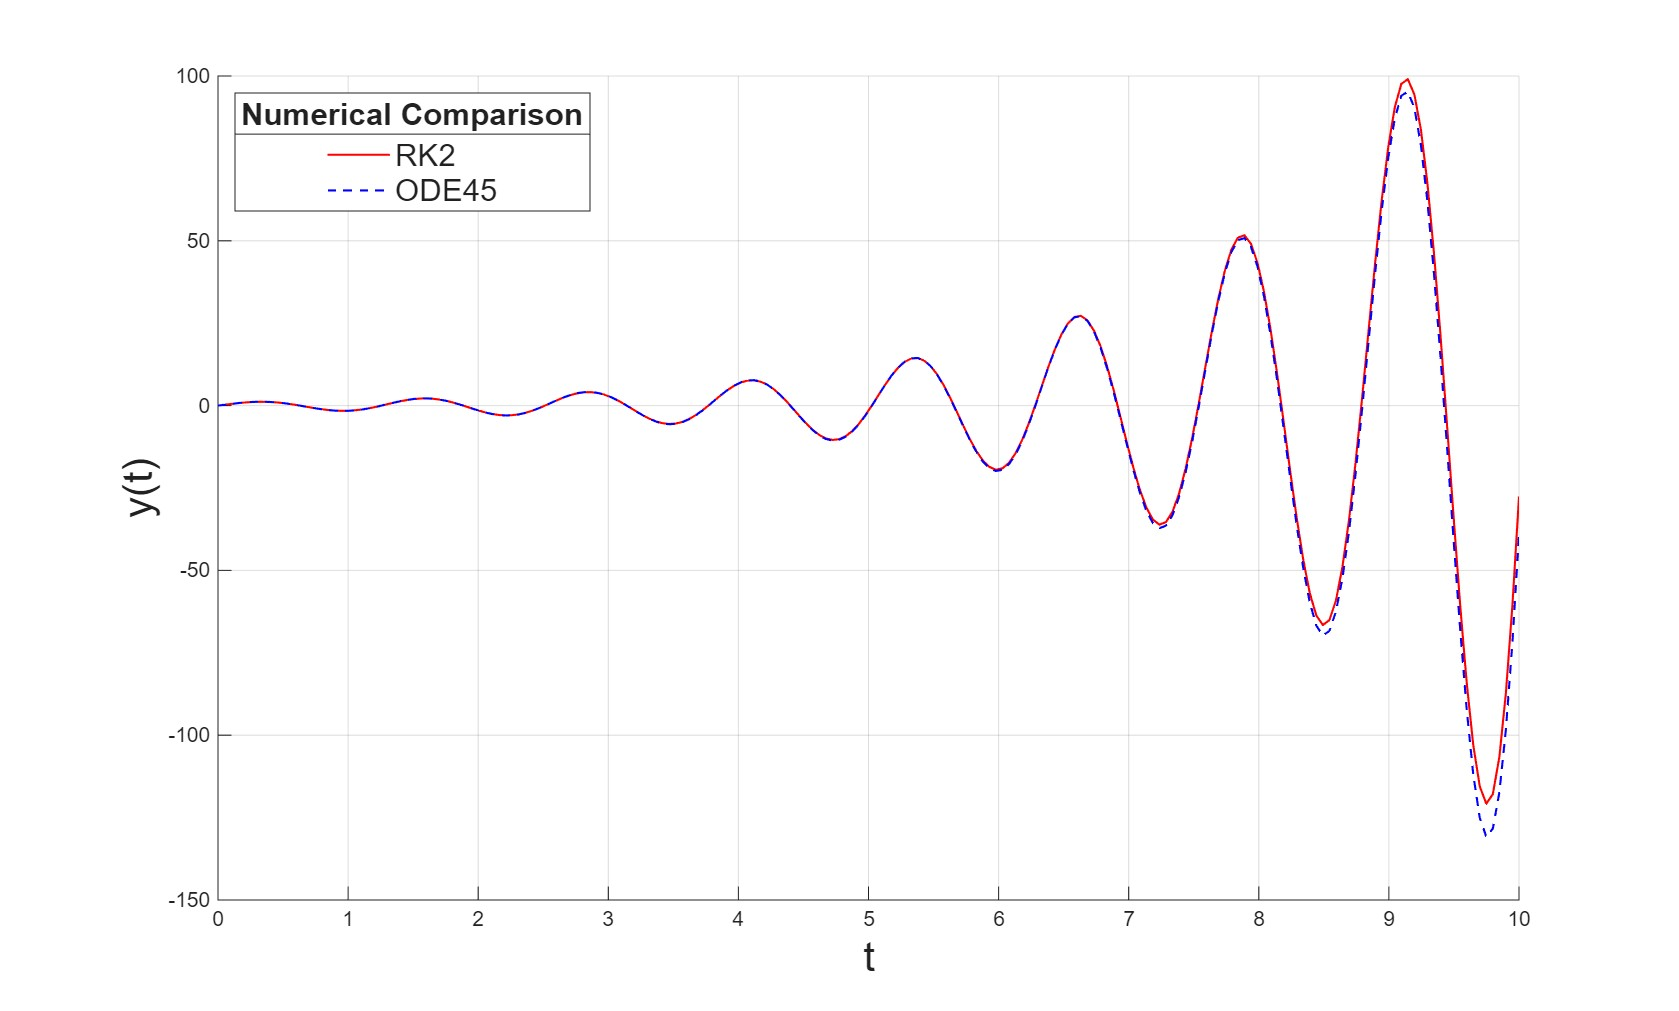
\includegraphics[width=1\linewidth]{rk2_005.jpg}
    \caption{RK2, h = 0.05}
    \label{fig:rk2_005}
\end{figure}
\begin{figure}[H]
    \centering
    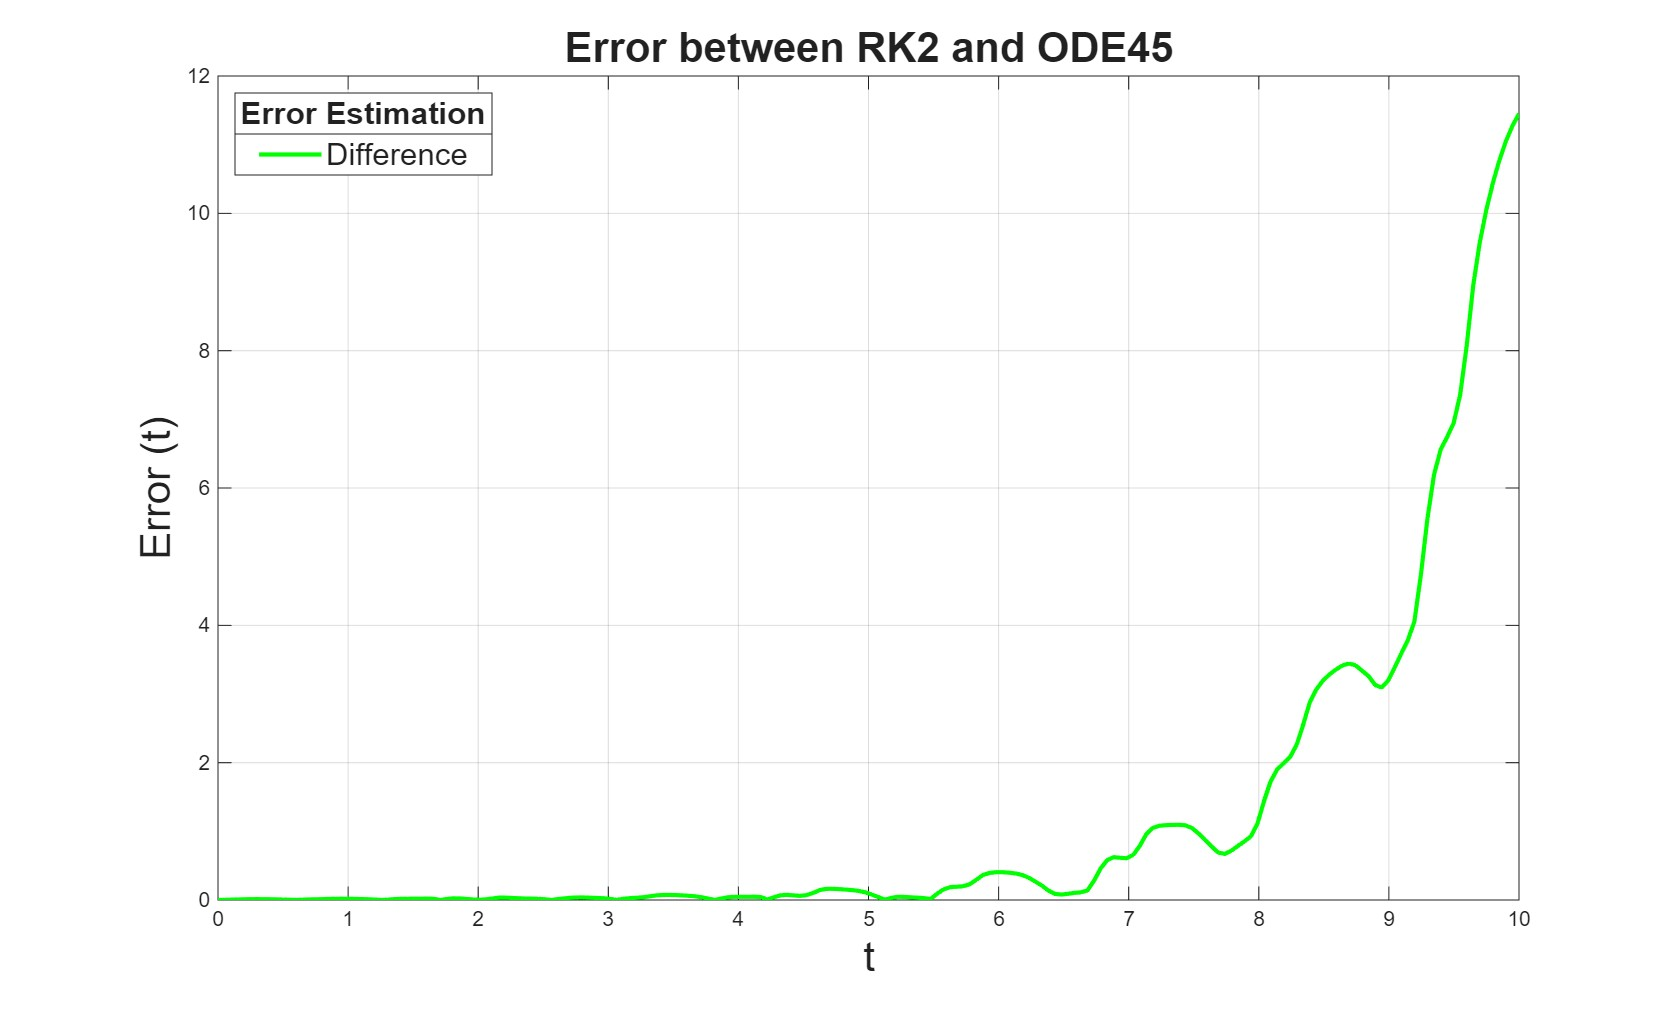
\includegraphics[width=1\linewidth]{error_rk2.jpg}
    \caption{Error RK2}
    \label{fig:error_rk2}
\end{figure}
The error in this case, we can see amounts to at most $12$. That is to be expected, as the method is supposed to be more accurate.
\section{RK4 Method}
Similar to RK2, RK4 has 4 coefficients which need to be calculated beforehand. This in turn makes the result more precise, but also require much more power to do so. The calculation is as follows:
\begin{align*}
    A = f(x_n, y_n)\\
    B = f(x_n + \frac{h}{2}, y_n + \frac{A}{2}h)\\
    C = f(x_n + \frac{h}{2}, y_n + \frac{B}{2}h)\\
    D = f(x_n + h, y_n + Ch)\\
    y_{n+1} = y_n + \frac{A+2B+2C+D}{6}h
\end{align*}
\begin{figure}[H]
    \centering
    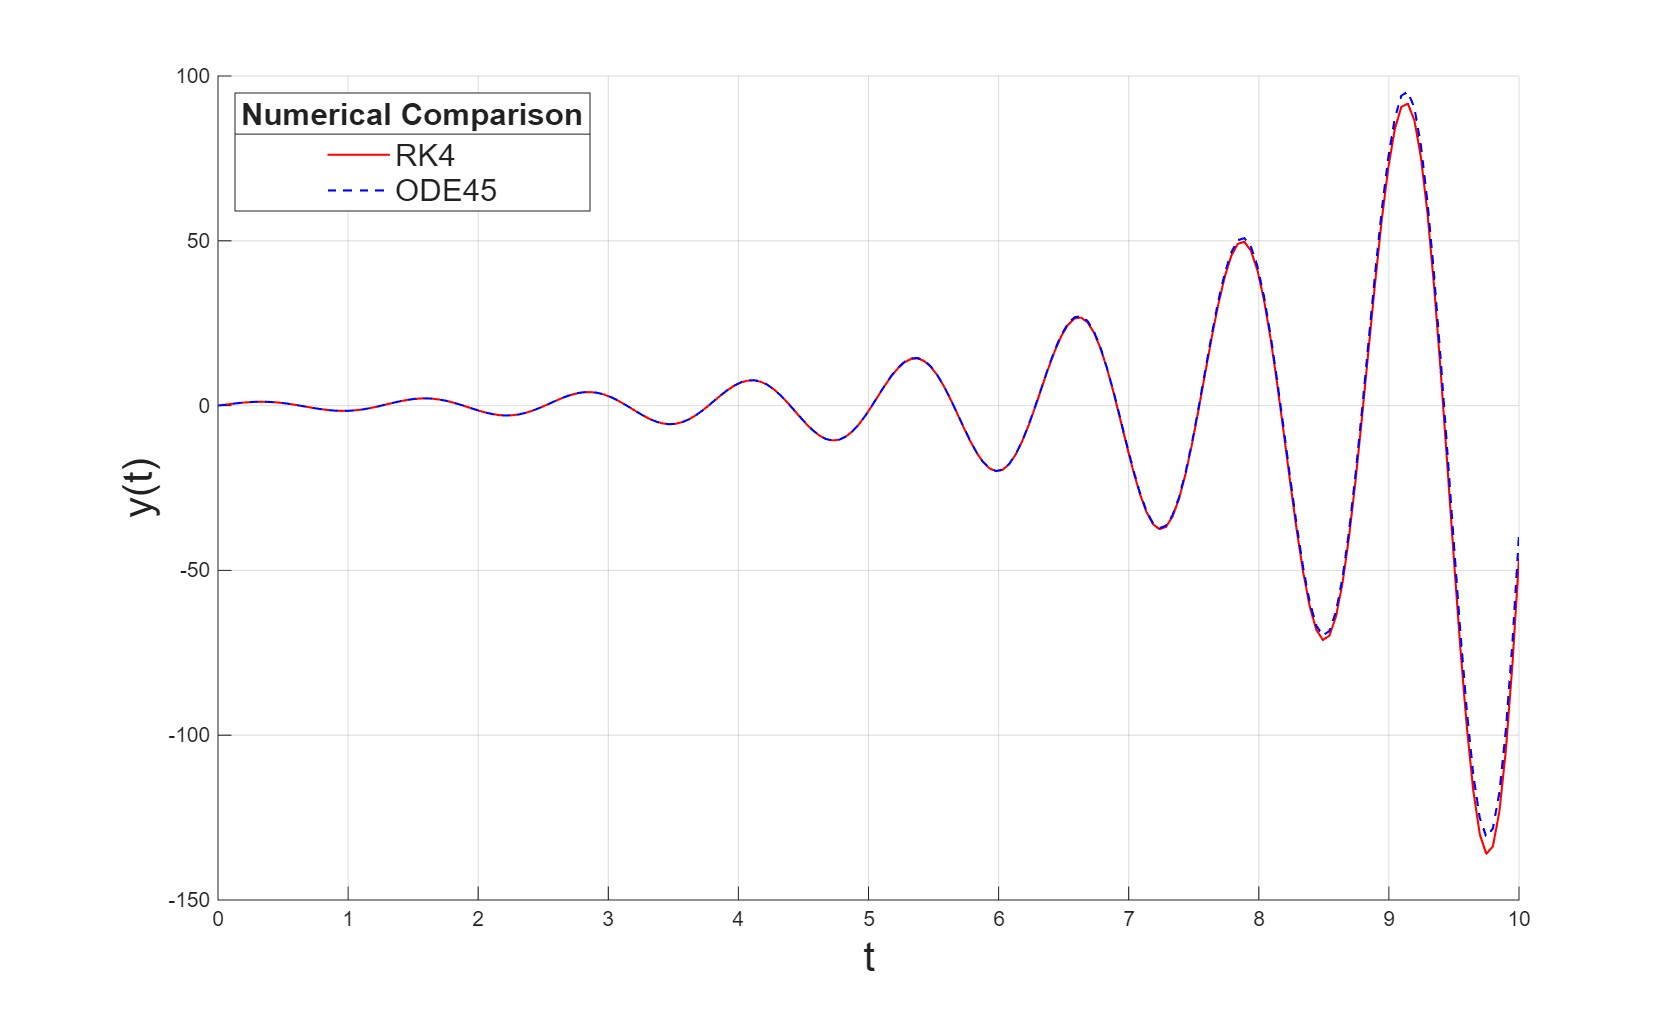
\includegraphics[width=1\linewidth]{rk4_005.jpg}
    \caption{RK4, h = 0.05}
    \label{fig:rk4_005}
\end{figure}
\begin{figure}[H]
    \centering
    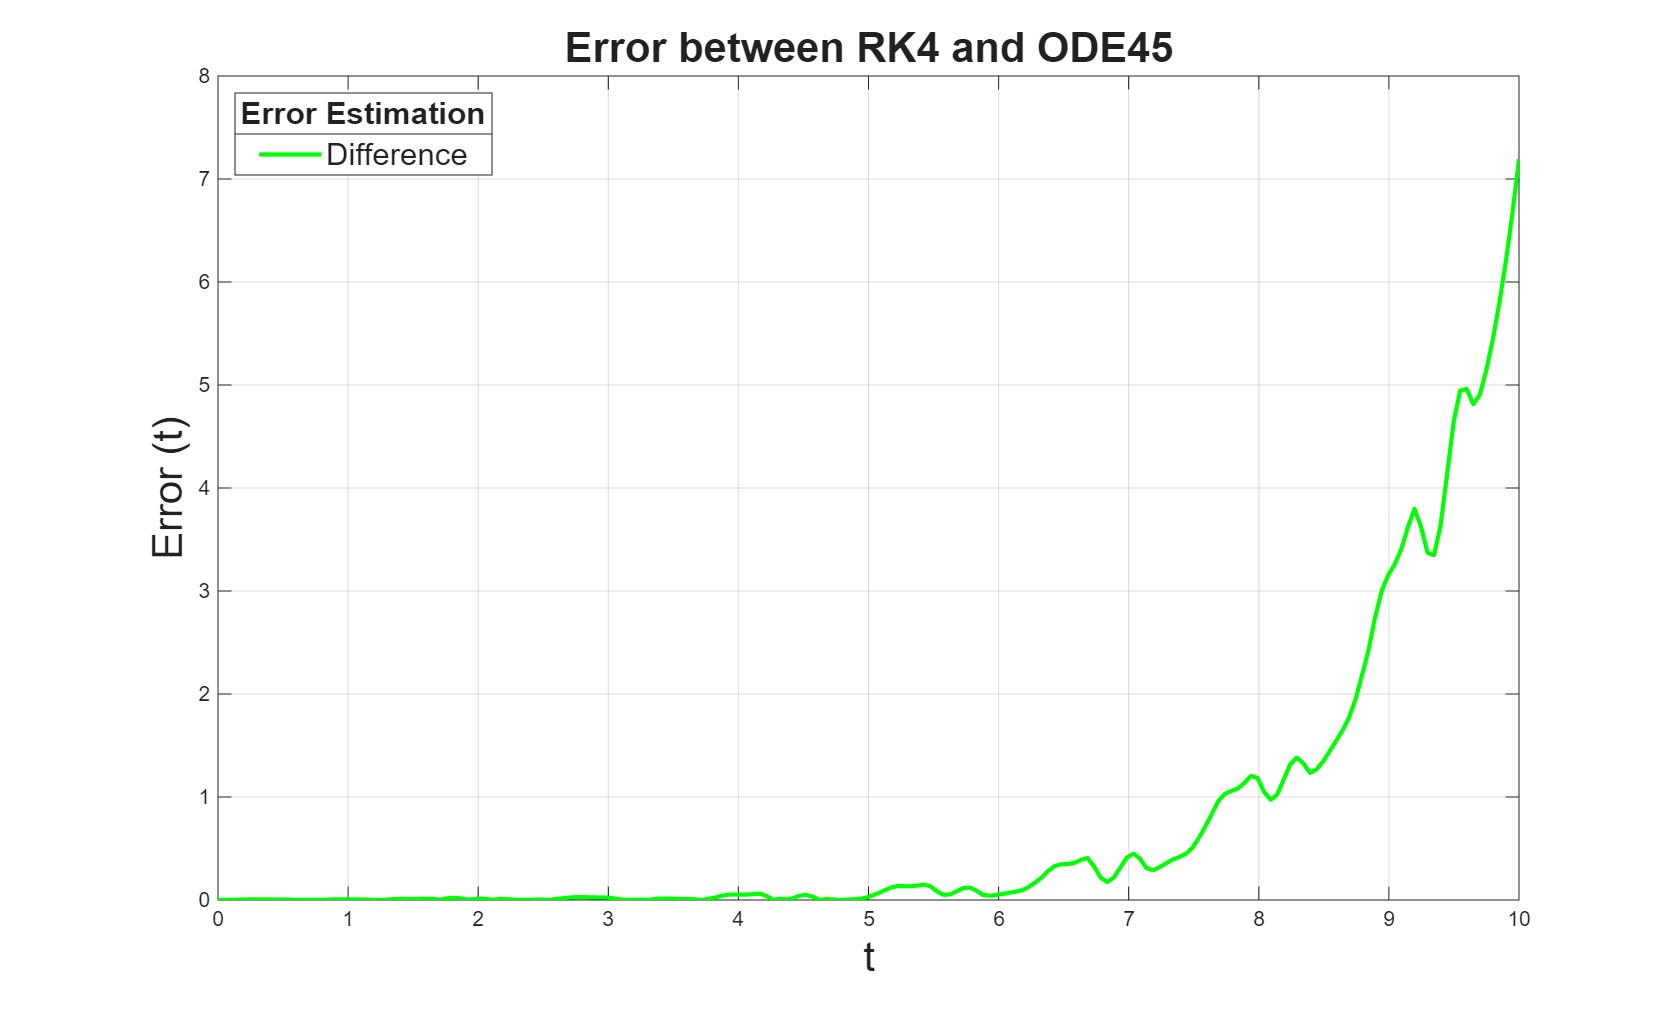
\includegraphics[width=1\linewidth]{error_rk4.jpg}
    \caption{Error RK4}
    \label{fig:error_rk4}
\end{figure}
This one is also more accurate than the previous, again expected. In this case, though the difference between the errors of RK2 and RK4 is noticably less than the error difference between RK1 and RK2. As a conclusion we can draw, that in this case the RK4 method is not needed as it requires too much computing power and does not reduce the error by that much. For the ODE in question RK2 is the perfect balance between calculation steps and accuracy.

\section{1-D Heat Equation MATLAB}
In this section I am showcasing a classic example of how numerical solutions are easier than the analytical ones. The Heat Equation describes the change of temperature with respect to $t$ of a system, in our case in a one dimensional rod with length $x$. \\
\textbf{Assumptions:}
\begin{itemize}
    \item Start and end points of the rod have a fixed temperature.
    \item We start with a initial temperature distribution.
    \item  The Partial Differential Equation (PDE), being solved is: $\frac{\partial u^2}{\partial^2x} = \alpha*\frac{\partial u}{\partial t}$.
    \item  The constant $\alpha$ is a physical constant $\alpha$ around $\approx (0, 2)$. 
\end{itemize}
To solve this problem the temperature needs to be determined at all possible points $u(x, t): \forall x, t$. With the given initial distribution we can numerically approximate the value of the second derivative with respect to x in all points on the rod:
\begin{equation*}
    u_{xx}(x, t) = \frac{u_x(x+dx, t) - u_x(x, t)}{dx} 
\end{equation*}
\begin{equation*}
    u_{xx}(x, t) = \frac{u(x+dx, t) - 2u(x, t) + u(x-dx, t)}{dx^2}
\end{equation*}
With approximation for the second derivative we can calculate the values for all points on the rod. To find the respective values for the first derivative with respect to time we use the PDE from the start. And to find the value of the temperature at the next moment in time we use the first derivative approximation as follows:
\begin{equation*}
    u_t(x, t) = \alpha u_{xx}(x, t)
\end{equation*}
\begin{equation*}
    u_t(x, t) = \frac{u(x, t+dt) - u(x, t)}{dt}
\end{equation*}
\begin{equation*} 
    \Rightarrow u(x, t+dt) = u_t(x, t)dt + u(x, t)
\end{equation*}
We repeat this algorithm for as long as we want. With the logic ready, all that is left is to implement it in MATLAB. After generating some random noise as input data we get the following results out:

\begin{figure}[H]
\begin{subfigure}[h]{0.49\linewidth}
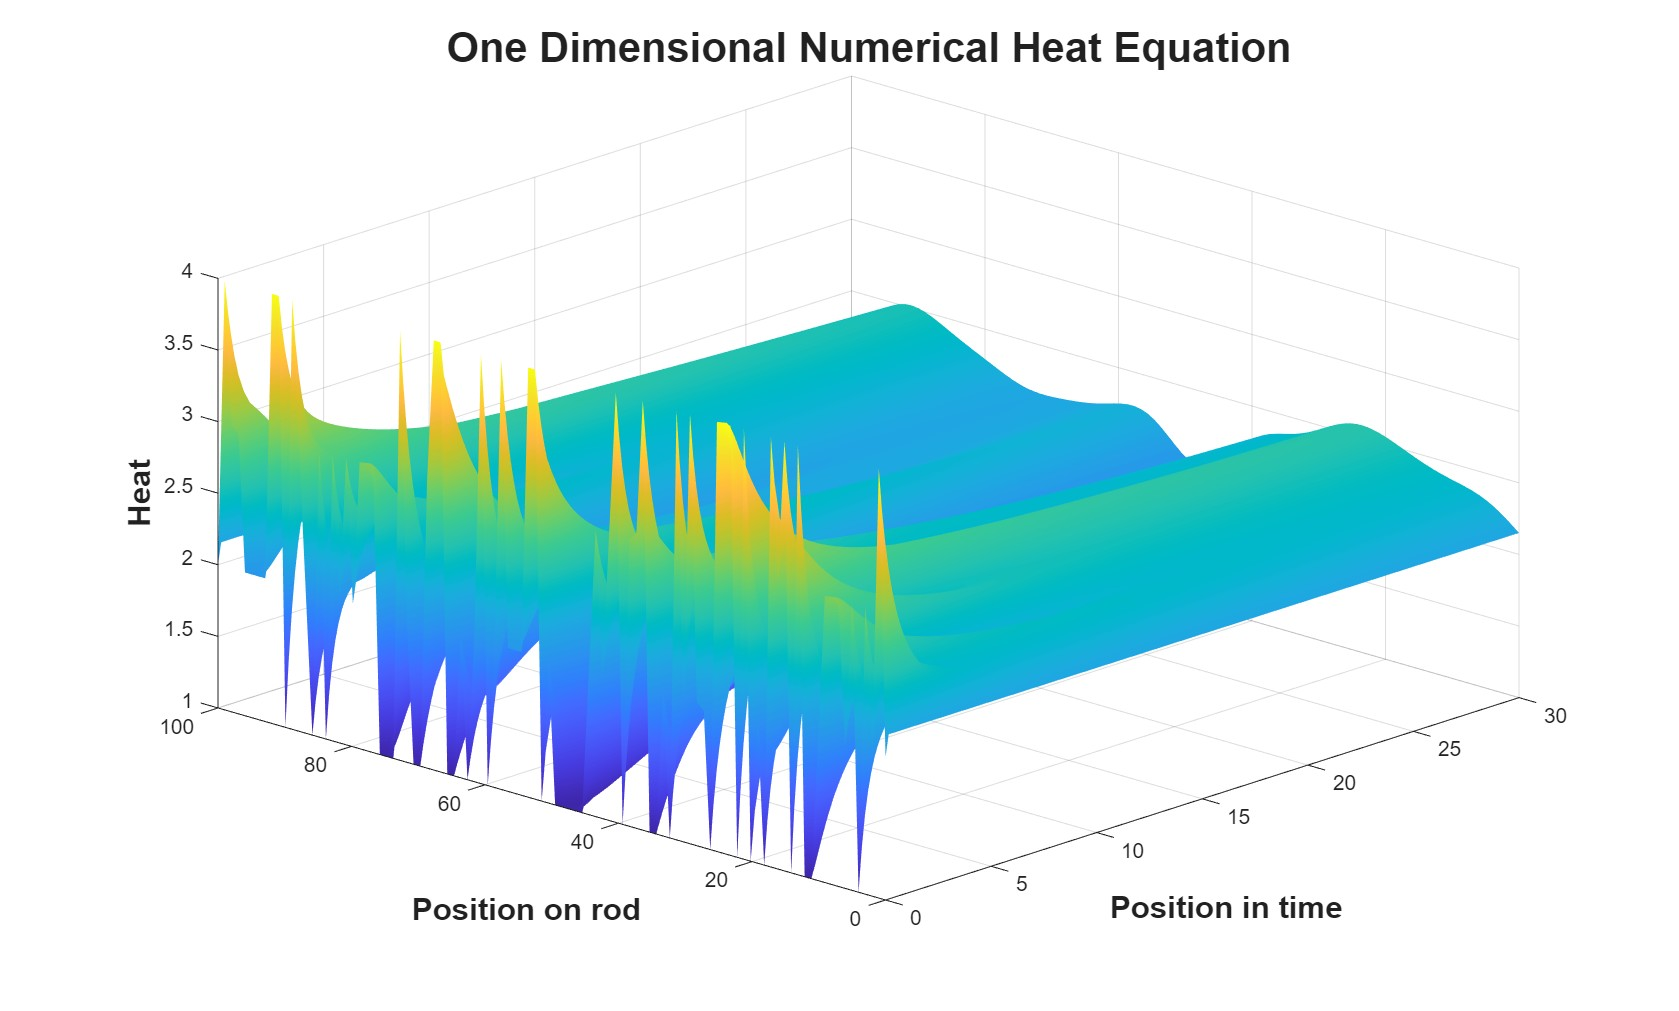
\includegraphics[width=\linewidth]{1d_example_front.jpg}
\caption{Front}
\end{subfigure}
\hfill
\begin{subfigure}[h]{0.49\linewidth}
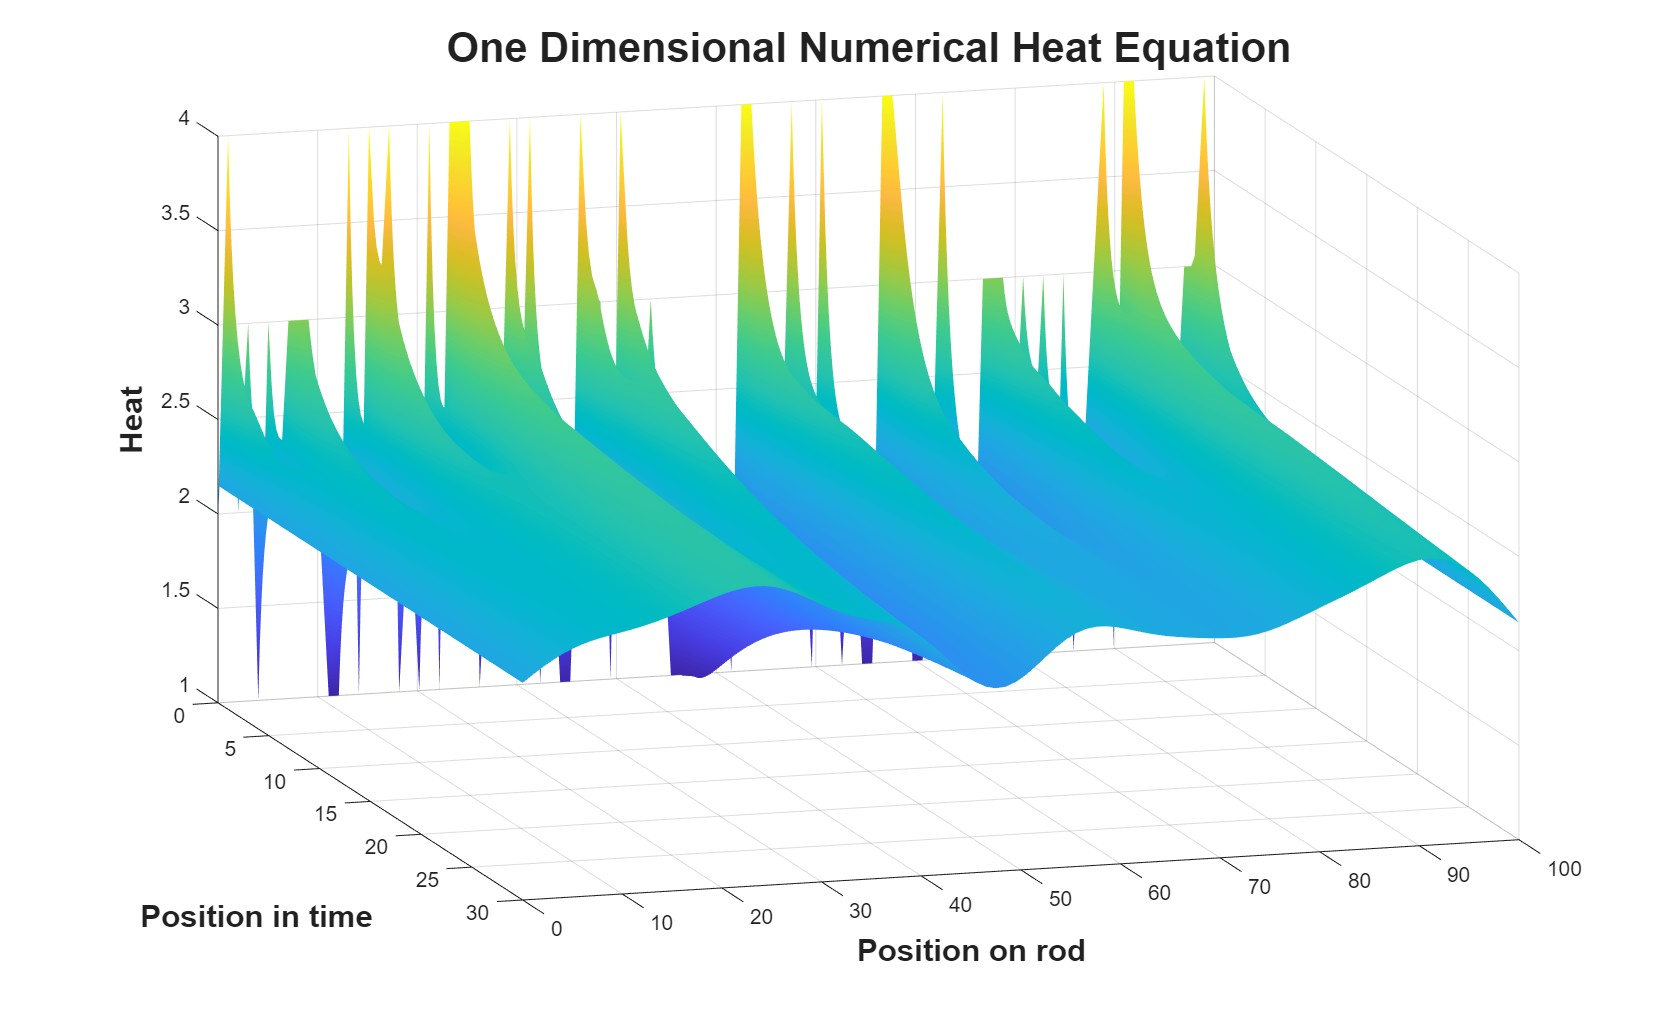
\includegraphics[width=\linewidth]{1d_example_back.jpg}
\caption{Back}
\end{subfigure}
\caption{Evolution in time for $\alpha = 0.5$}
\end{figure}

\begin{figure}[H]
\begin{subfigure}[h]{0.49\linewidth}
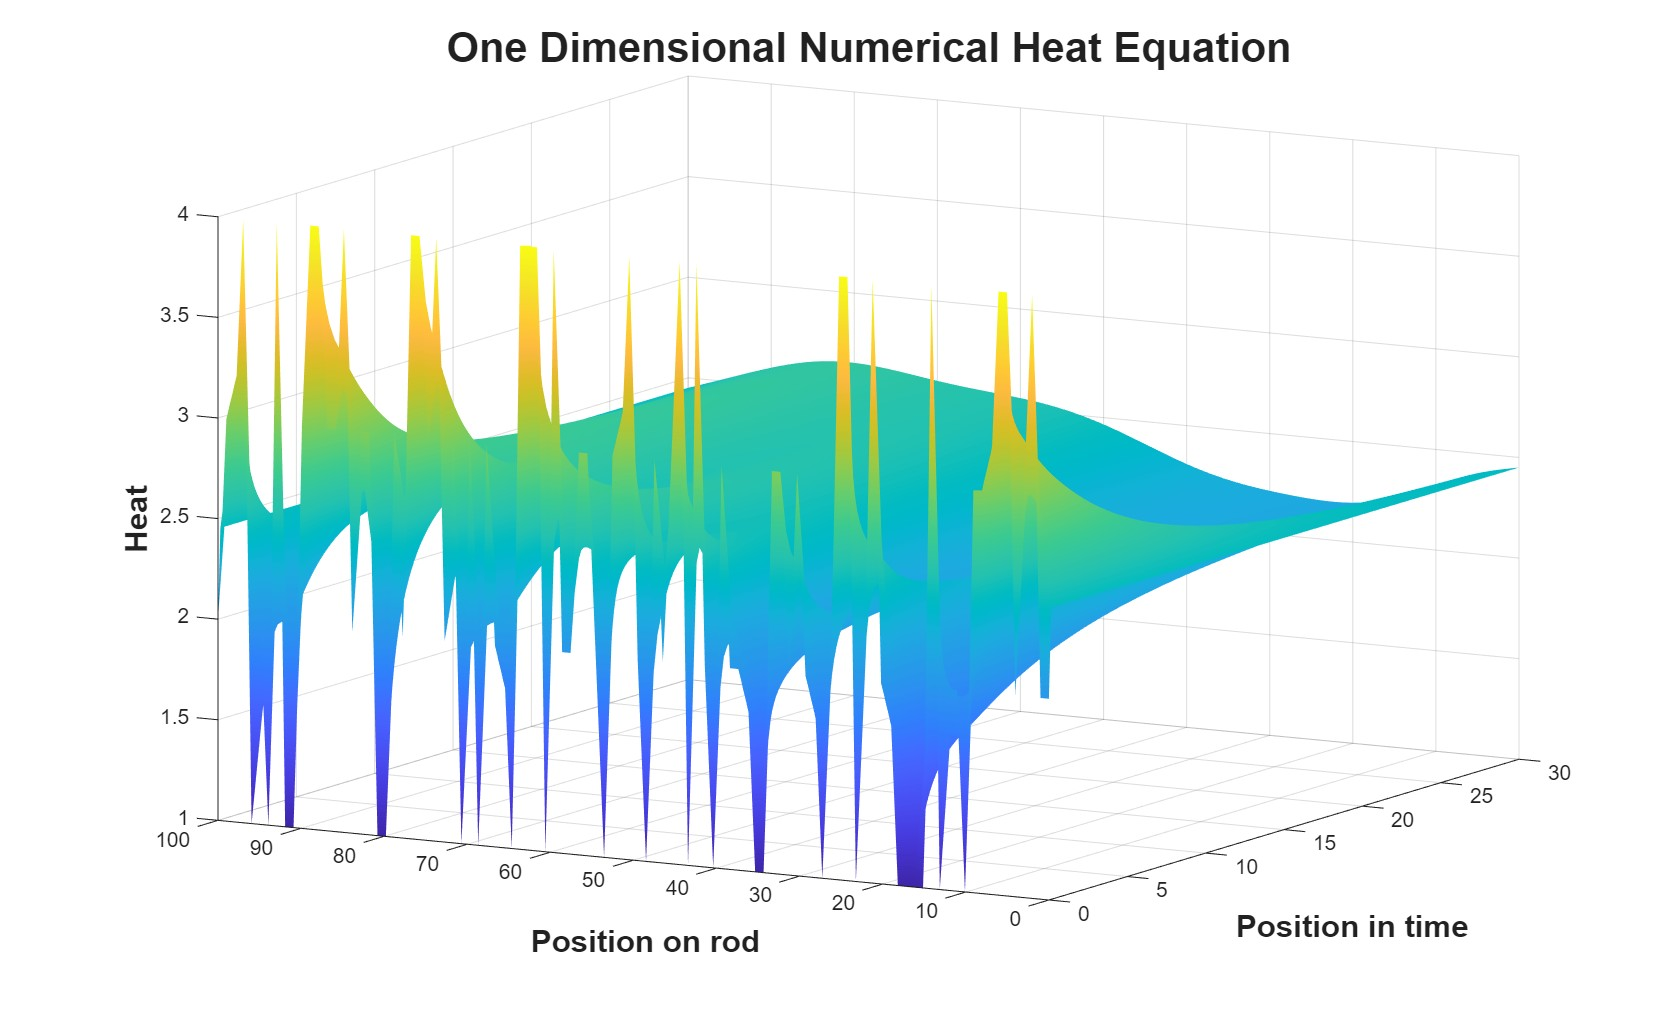
\includegraphics[width=\linewidth]{1d_heat_example_high_front.jpg}
\caption{Front}
\end{subfigure}
\hfill
\begin{subfigure}[h]{0.49\linewidth}
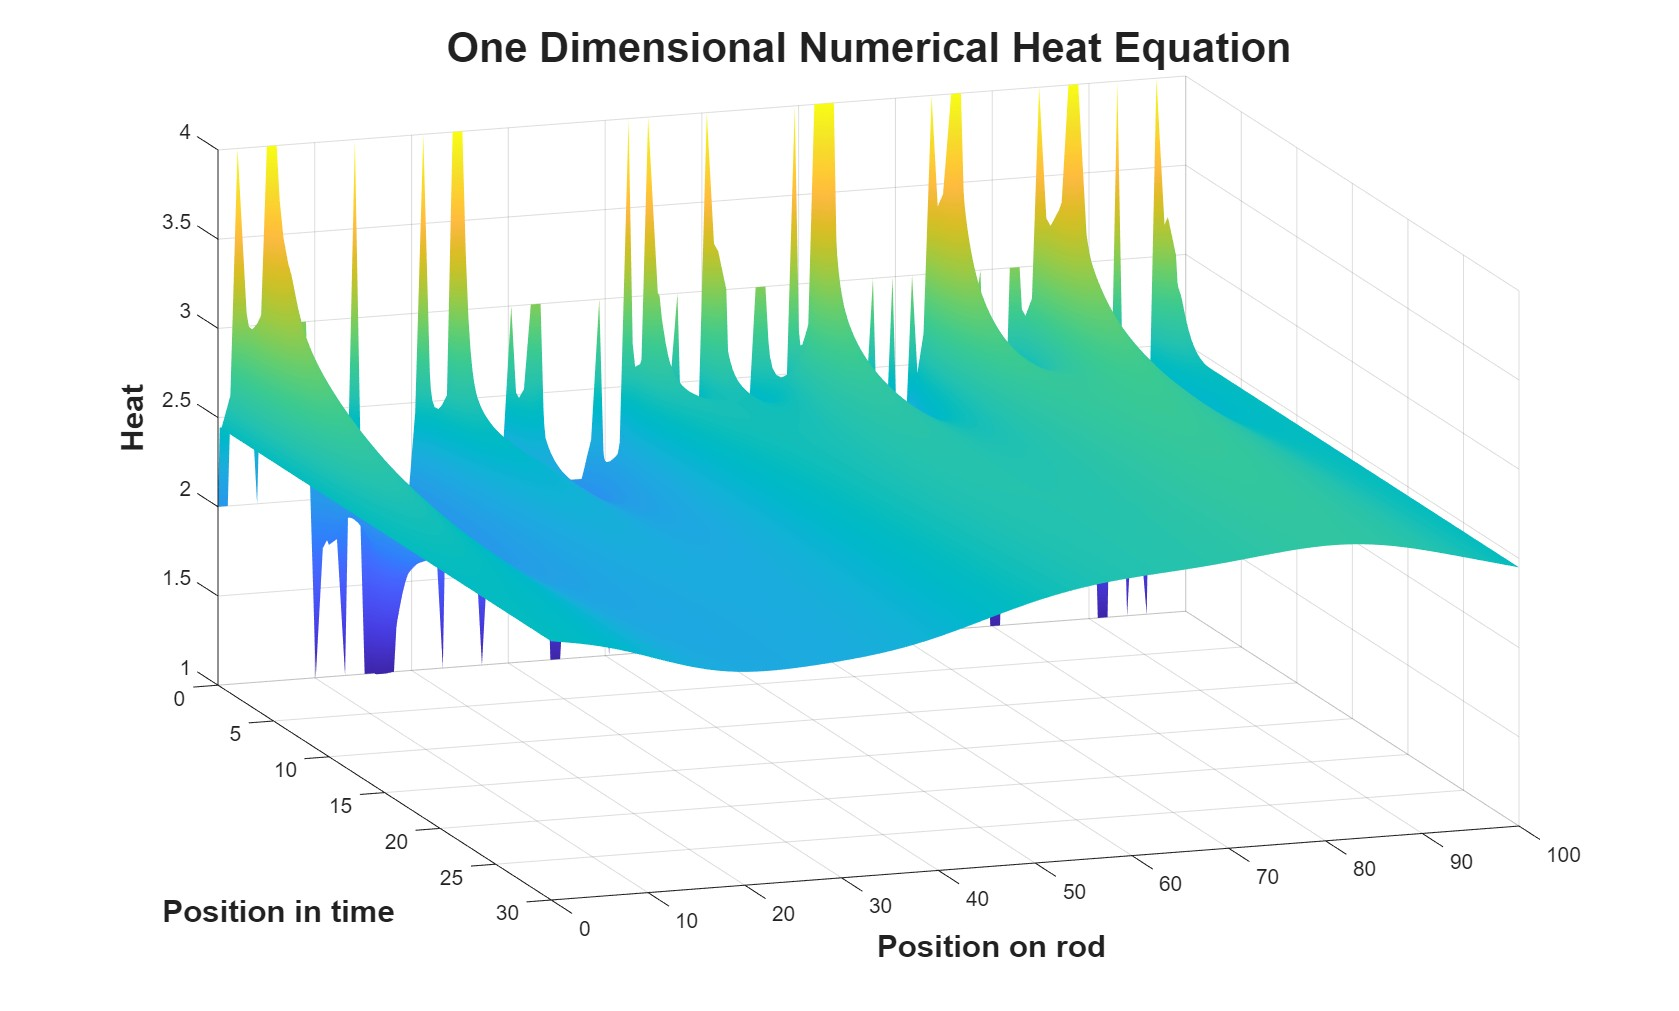
\includegraphics[width=\linewidth]{1d_heat_example_high_back.jpg}
\caption{Back}
\end{subfigure}
\caption{Evolution in time for $\alpha = 1.5$}
\end{figure}
Naturally if we increase the constant, the desired results appear faster and with lower amount of iterations. The problem arises, if we increase the constant too much without readjusting the other input parameters. The result diverges into nonsensical values, which are a result of not respecting the limit for the stability of the solution: $\alpha \leq \frac{dx^2}{2dt}$.


\section{Neville Interpolation}
This section focuses on one algorithm, used for interpolation.
Neville's algorithm requires as input a vector of $x$ and a vector of $y$ data, as well as a starting $x_0$ point.
The data corresponds to a set of points on the cartesian plane.
What comes as output is the predicted $y_0$ value at the $x_0$ coordinate.
The predicition is based on a polynomial function with a degree one less than the size of the data set.
The algorithm recursively approximates each time a higher order polynomial to fit all points from the set.
The recursive formula is as follows:
\begin{equation*}
    P_{i, j} = \frac{(x_0 - x_i)*P_{i+1,j-1} - (x_0 - x_{i+j-1})*P_{i, j-1}}{x_{i+j-1} - x_i}
\end{equation*}
That is the equation for the algorithm, implemented in MATLAB.
The theory behind is more complicated. Let us look at an example with only 3 points.
\begin{equation*}
    x = [1, 2, 3] \hspace{1cm} y = [1, 4, 9]
\end{equation*}
We want to find the value at $x_0 = 2.5$.
The start values are $P_{i, 0} = y_i$. That approximates the polynomial to a constant function.
Of course that is far from ideal as shown in Figure \ref{fig:neville_const}. 
\begin{figure}[H]
    \centering
    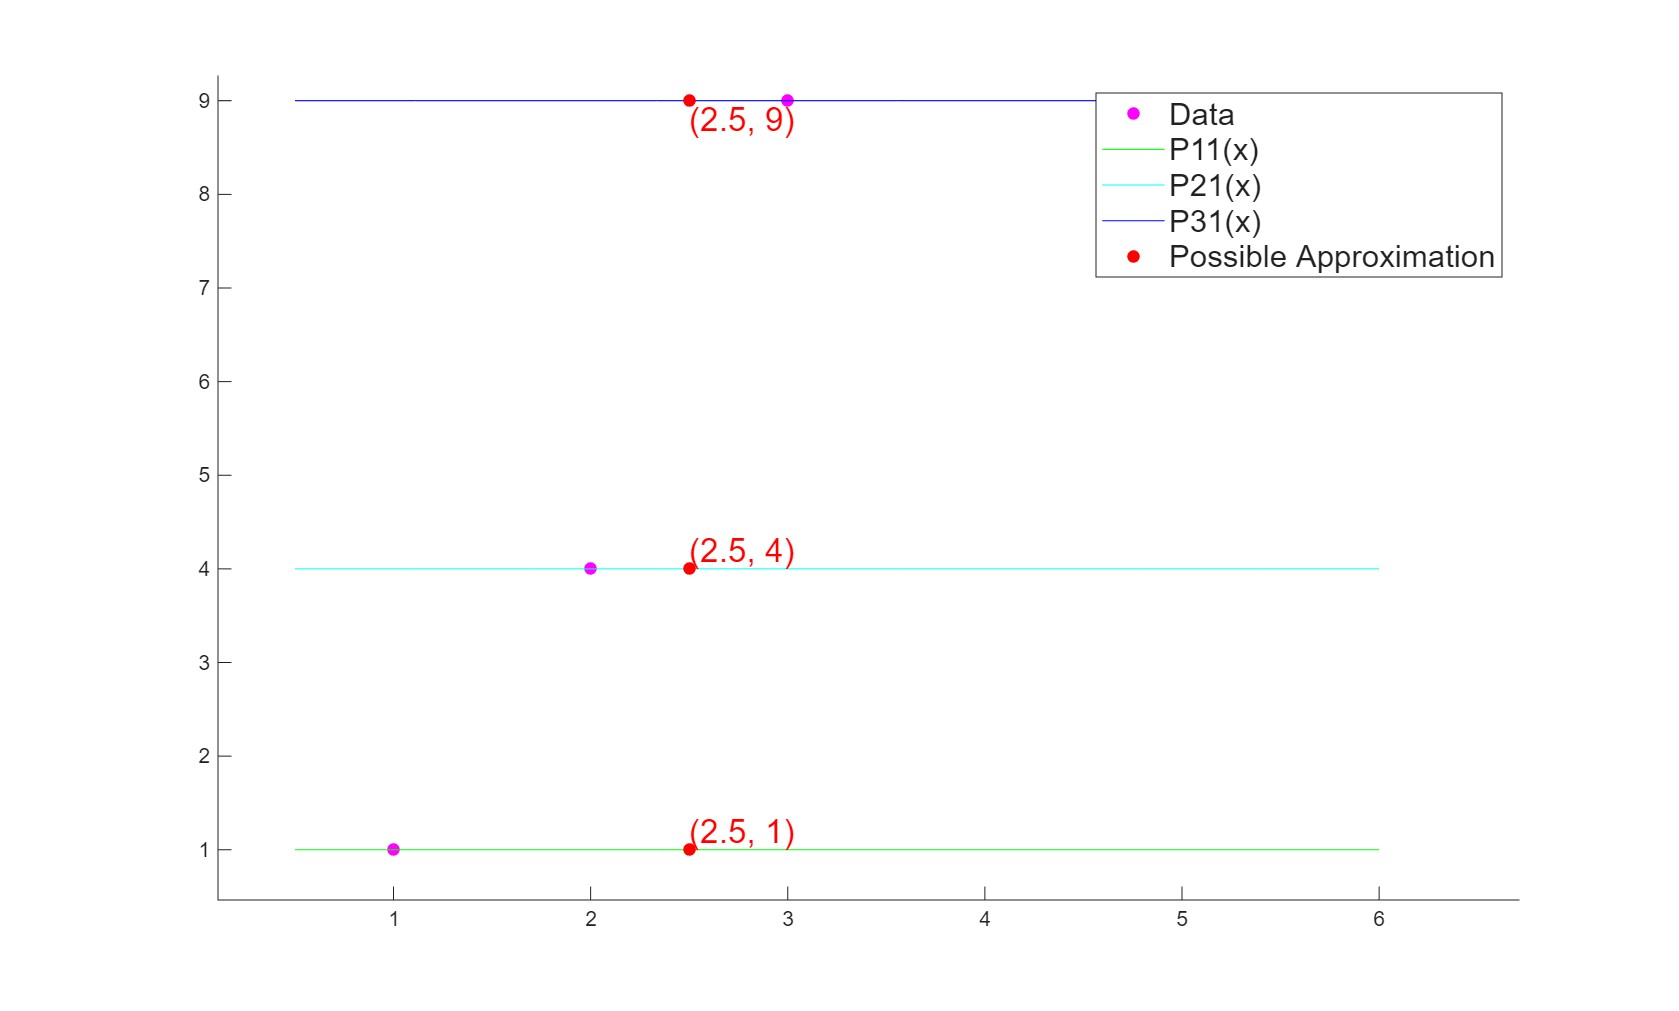
\includegraphics[width=1\linewidth]{neville_3p_const.jpg}
    \caption{Constant Approximation}
    \label{fig:neville_const}
\end{figure}
Using the algorithm again we get the following 2 values: $P_{1, 2} = 5.5$ and $P_{2, 2} = 6.5$.
If instead of $x_0$ we just use $x$ as a variable we get not values but 2 line equations: $P_{1, 2} = 3x-2$ and $P_{2, 2} = 5x -6$.
The lines are closer but still not good enough, as seen in Figure \ref{fig:neville_lin}.
\begin{figure}
    \centering
    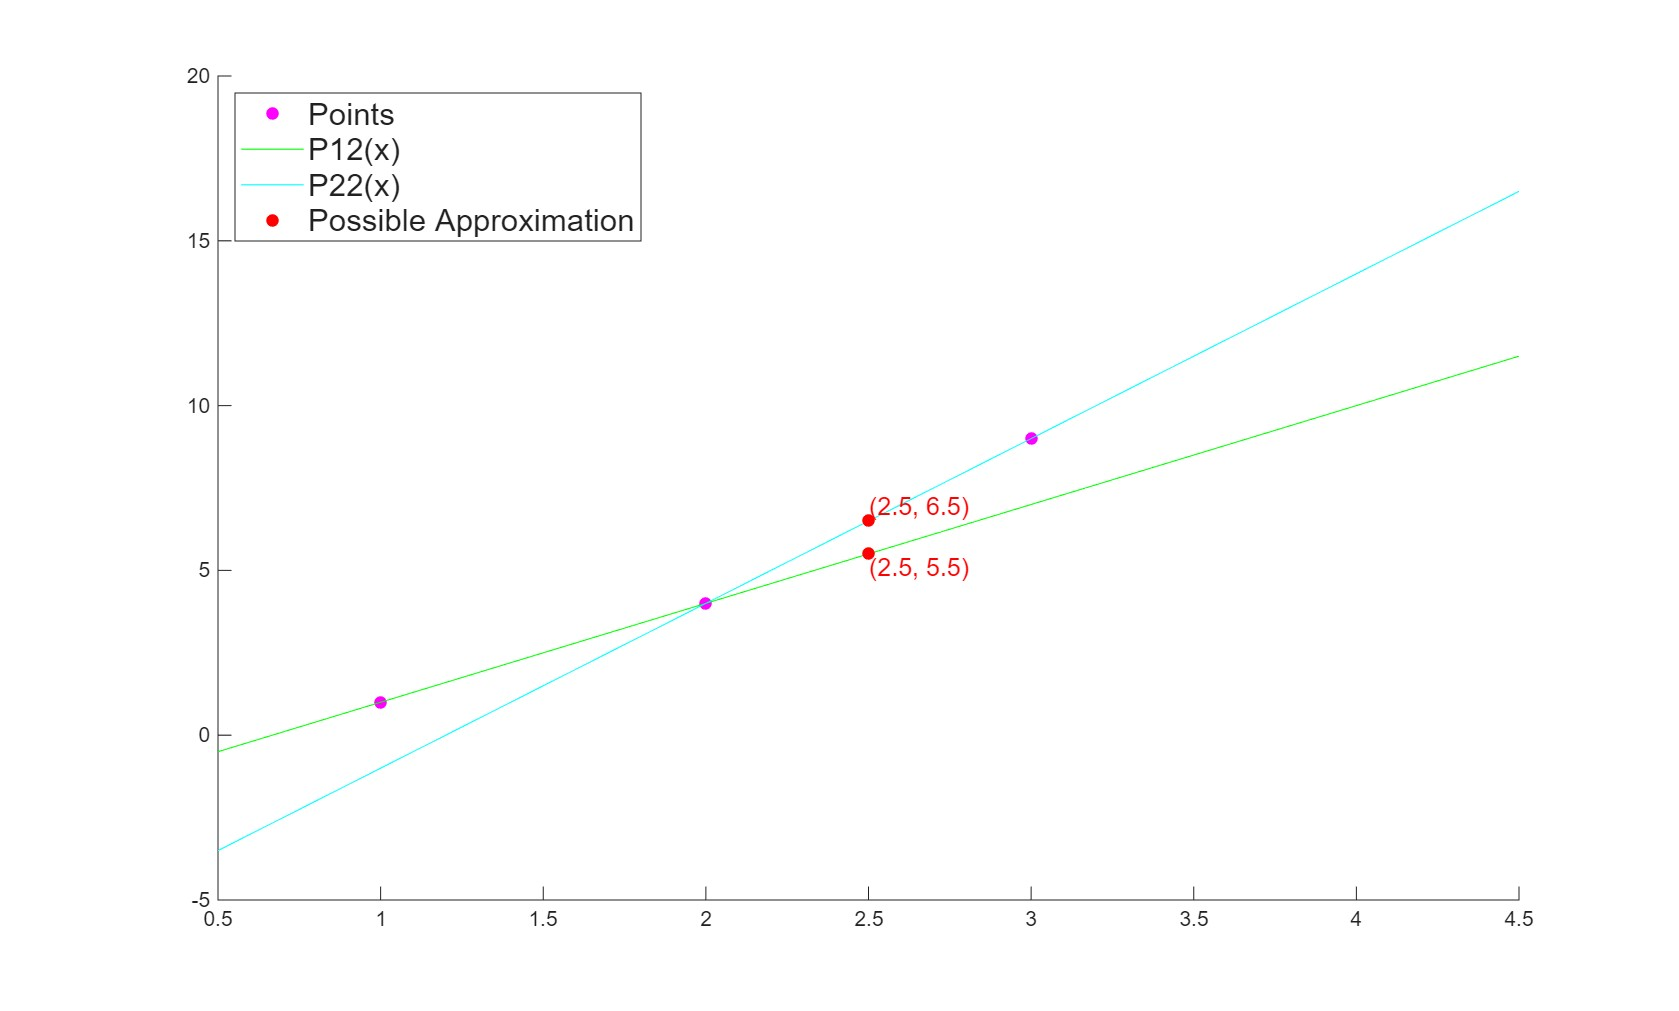
\includegraphics[width=1\linewidth]{neville_3p_lin.jpg}
    \caption{Linear Approximation}
    \label{fig:neville_lin}
\end{figure}
\begin{figure}[H]
    \centering
    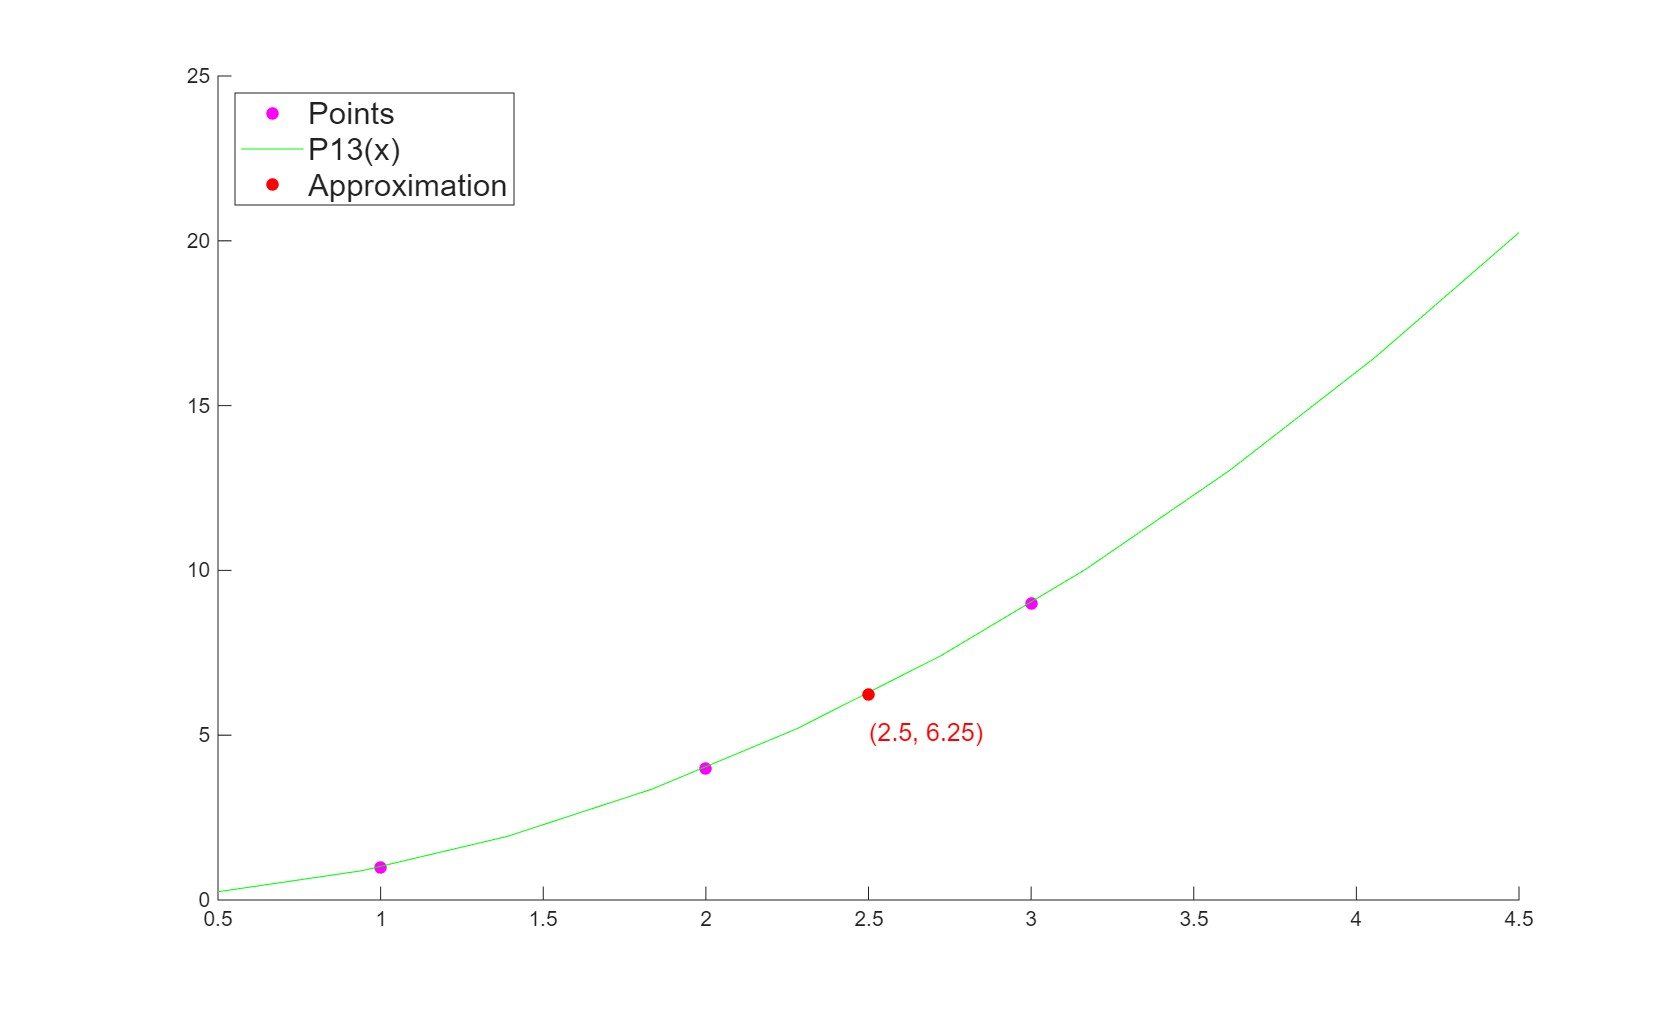
\includegraphics[width=1\linewidth]{neville_3p_qudr.jpg}
    \caption{Quadratic Approximation}
    \label{fig:neville_qudr}
\end{figure}
\newpage
Doing this one last time we get the final $P_{1, 3} = 6.25$.
If we used the $x$ instead of $x_0$ we get the polynomial: $P_{1, 3} = x^2$. If we substitute with $x_0$
we get the value which our algorithm would have given, as illustrated in Figure \ref{fig:neville_qudr}.
This can be summarized very nicely in a table: \\
\begin{table}[H]
    \centering
    \begin{tabular}{|c|c|c|c|}
        \hline 
        &j=1&j=2&j=3\\ \hline
    i=1&$P_{1, 1} = 1$&$P_{1, 2} = 5.5$&$P_{1, 3} = 6.25$ \\
    i=2&$P_{2, 1} = 4$ & $P_{2, 2} = 6.5$ & X \\
    i=3&$P_{3, 1} = 9$ & X & X \\   
    \hline 
    \end{tabular} 
    \caption{Table Representaiton of Neville's Algorithm}   
    \label{table:neville_tbl}
\end{table}




\section{Trapezoidal Integration}

\section{References WIP}
\begin{itemize}
    \item mit ode kurs
    \item MATLAB helpa
    \item 3b1b youtube videoto za 1dheat
    \item $https://www.cs.princeton.edu/courses/archive/fall11/cos323/notes/cos323_f11_lecture19_pde2.pdf$
\end{itemize}

\end{document}
